%! Author = mr
%! Date = 3/13/2025
%%% Abstract
\begin{abstract}
    The Vortex Æther Model (VAM) introduces a unified, non-relativistic theoretical framework wherein gravity, electromagnetism, and quantum phenomena arise from structured vorticity within an inviscid superfluid-like Æther. Unlike General Relativity, which depends on four-dimensional spacetime curvature, VAM proposes that stable vortex knots in three-dimensional Euclidean space generate fundamental forces and quantized states through fluid dynamics and vortex topology. Central to this model is absolute universal time, where observed time dilation results from vortex-induced local energy gradients rather than relativistic effects. VAM yields experimentally testable predictions, including superfluid analogs of frame-dragging, magnetic fields in electrically neutral fluids, and atomic-scale quantization phenomena akin to those observed in helium II. Fundamental constants such as the vortex-core tangential velocity $C_e$ and the Coulomb barrier radius $r_c$ anchor core rotation speeds and interaction strengths, providing explicit testable parameters for experimental verification.
\end{abstract}

\maketitle

\begin{figure}[h]
    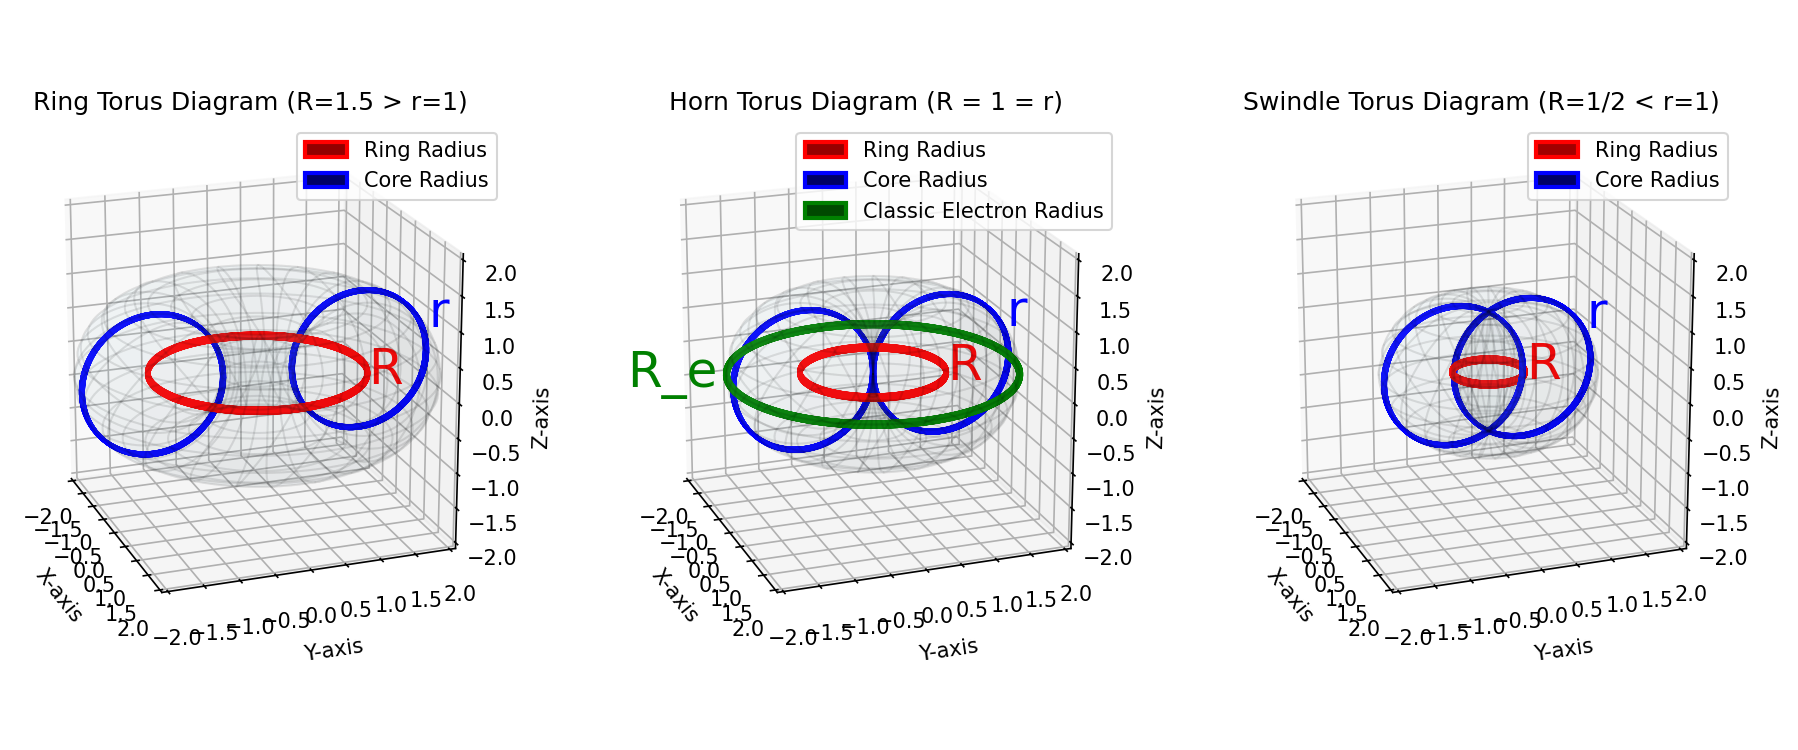
\includegraphics[width=\textwidth]{torus}
    \caption{Illustration of a vortex filament in Æther.}
    \label{fig:vortex}
\end{figure}


\section{Introduction}

The concept of an all-pervading Æther has profoundly influenced physics since the 19th century, notably with James Clerk Maxwell’s proposal that electromagnetic waves necessitate a propagating medium~\cite{Maxwell1865}. However, early experiments, particularly Michelson and Morley's \cite{michelson1887}, failed to detect the classical stationary Æther, leading Einstein to replace it with the invariant speed of light and spacetime geometry of Special and General Relativity~\cite{einstein1916foundation}.

Nevertheless, recent developments in quantum field theory and experimental studies of quantum superfluids, notably helium II, demonstrate that even the vacuum may exhibit nontrivial fluid-like properties, including quantized vortices and discrete energy states~\cite{Wilczek1999,Donnelly1991quantized}. Inspired by these developments and the historical ideas of Helmholtz~\cite{helmholtz1867integrals}, Kelvin~\cite{kelvin1867vortex}, and Maxwell~\cite{Maxwell1865}, the Vortex Æther Model (VAM) revisits the Æther hypothesis, proposing an inviscid, incompressible superfluid medium whose structured vortices underpin all fundamental physical phenomena.

VAM posits that gravitational attraction emerges from vortex-induced pressure gradients analogous to Bernoulli’s principle rather than spacetime curvature. Similarly, electromagnetic phenomena are explained by vortex topology, where stable knotted vortices form analogs to charges and currents without necessitating discrete force carriers or additional dimensions. Quantum effects, including energy quantization and wave-particle duality, are interpreted through conserved vortex helicity and stable vortex knots, linking macroscopic fluid dynamics directly to microscopic quantum states.

Crucially, VAM reinstates absolute universal time, with observed time dilation effects resulting from local variations in vortex-induced energy distributions rather than relativistic velocity-based distortions. This provides an elegant explanation of phenomena traditionally associated with relativistic physics, such as gravitational lensing and frame-dragging, as natural outcomes of vortex circulation.

This paper presents the foundational principles and novel mathematical formalism of VAM, explicitly deriving key physical constants and demonstrating their implications. Furthermore, it highlights experimental tests uniquely predicted by this model, including analogs of gravitational frame-dragging in superfluids, electromagnetic phenomena in charge-neutral fluids, and measurable quantum effects arising from structured vortex configurations. By integrating classical fluid mechanics, quantum principles, and electromagnetic theory within a purely three-dimensional framework, VAM provides a coherent, testable alternative to contemporary physics paradigms.

The subsequent sections systematically present the mathematical formalism and specific experimental predictions, positioning VAM as a cohesive, empirically falsifiable alternative theory of fundamental interactions.